\appendix
\section{Segmentation}


\begin{figure}[ht]
	\centering
	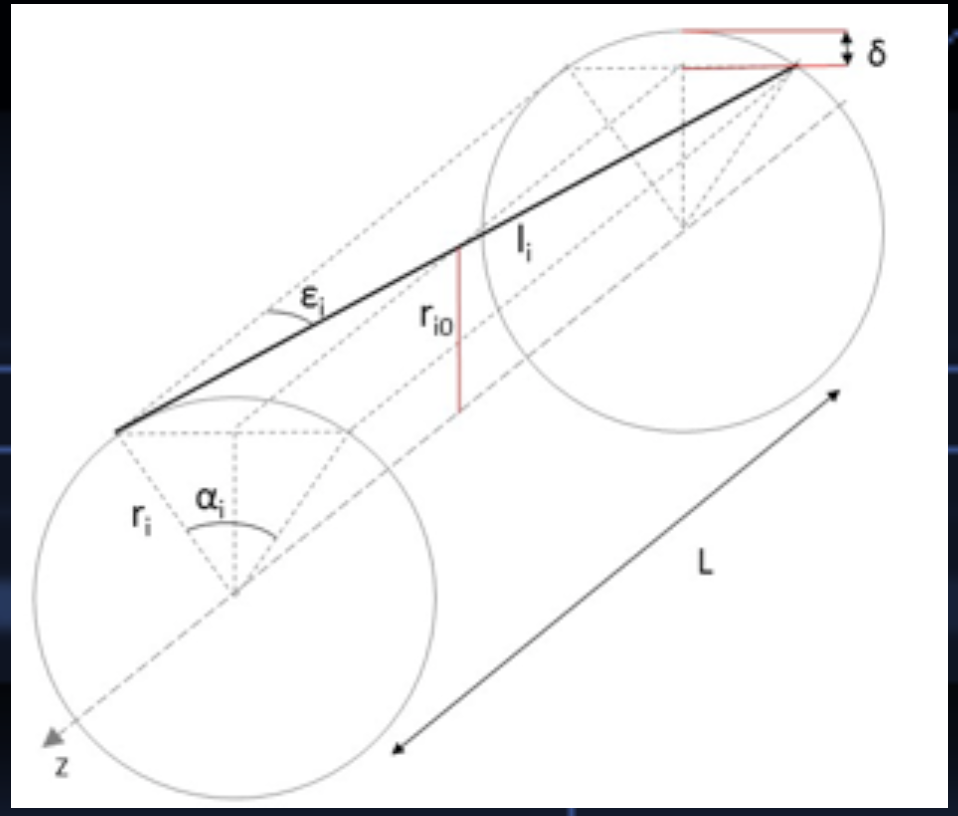
\includegraphics[width=0.6\textwidth]{figures/wires_DCH.png}%
	\caption{.}
	\label{wires_dch}
\end{figure}


\begin{figure}[ht]
	\centering
  \begin{tikzpicture}[scale=0.8]

    \pgfmathsetmacro{\R}{2}
    \pgfmathsetmacro{\wireAng}{45}

    \coordinate (O) at (0,0);
    \foreach \angle in
    {45,135}
    {
      \fill (\angle:\R) circle (0.1cm);
    }
    \draw (0,0) circle (\R);

    \draw[red]
    (\wireAng:\R) coordinate (wire1) --
    (3*\wireAng:\R) coordinate (wire2)
    pic [draw,->,angle radius=1cm,"$\alpha$", red] {angle = wire1--O--wire2};

    \draw
    (\R,0) coordinate (xcoord) --
    node[midway,below] {R} (O) --
    (\wireAng:\R) coordinate (slcoord)
    pic [draw,->,angle radius=1cm,"$\phi$"] {angle = xcoord--O--slcoord};

    \draw[-] (O) -- (wire2);

    \node[draw=none, right] at (wire1) {$w_{start}$};
    \node[draw=none, right, red] at (wire2) {$\Delta a$};
    \node[draw=none, left] at (wire2) {$w_{end}$};

    \begin{scope}[]
      \draw[->] (-2.5,0) -- (2.5,0) node[right] {$x$};
      \draw[->] (0,-2.5) -- (0,2.5) node[above] {$y$};
    \end{scope}
  \end{tikzpicture}
	\caption{.}
	\label{}
\end{figure}

\begin{equation}
  \Delta a = L \cdot \tan(\epsilon)
\end{equation}


\begin{equation}
  \alpha = 2 \cdot \arcsin\left({{L \cdot \tan(\epsilon)} \over {2
        \cdot R}}\right)
\end{equation}


\begin{itemize}
\item $\phi_{start}=\phi$
\item $\phi_{end}=\phi+\alpha$
  \begin{itemize}
  \item If $\epsilon<0 \Rightarrow \alpha<0$
  \end{itemize}
\end{itemize}

\begin{equation}
  \vec{w}_{start} = \begin{pmatrix}
    R \cos(\phi_{start}) \\
    R \sin(\phi_{start}) \\
    L/2
  \end{pmatrix}
\end{equation}

\begin{equation}
  \vec{w}_{end} = \begin{pmatrix}
    R \cos(\phi_{end}) \\
    R \sin(\phi_{end}) \\
    -L/2
  \end{pmatrix}
\end{equation}
